\documentclass[11pt]{article}
\usepackage{hyperref}
\usepackage{natbib}
\usepackage{amsmath}
\usepackage{nicefrac}
\usepackage[usenames,dvipsnames]{xcolor}
\usepackage{graphicx}
\usepackage{footnote}
\usepackage{rotating}
\usepackage{slashbox}
\usepackage{afterpage}
\usepackage{float}
\citestyle{mbe}
%%%%%%%%%%%%%%%%%%%%%%%%%%%%%%%%%%%%%%%%%%%%%%%%%%%%%%%%%%%%%%%%%%%%%%%%%%%%
%force setting figures at the top of the page:
    \makeatletter
    \setlength{\@fptop}{0pt}
    \makeatother
%%%%%%%%%%%%%%%%%%%%%%%%%%%%%%%%%%%%%%%%%%%%%%%%%%%%%%%%%%%%%%%%%%%%%%%%%%%%
%  personal abbreviations and macros
%    the following package contains macros used in this document:
%\input econfmacros.tex
%%%%%%%%%%%%%%%%%%%%%%%%%%%%%%%%%%%%%%%%%%%%%%%%%%%%%%%%%%%%%%%%%%%%%%%%%%%
\textwidth=6.9in  \textheight=9.6in
%%  Adjust these for your printer:
\leftmargin=-5in   \topmargin=-0.8in
\hoffset = -0.95in  \voffset = 0pt
\marginparwidth = 0pt
%% preprint number data:
%\newcommand\pubnumber{Article 14 in eConf C1304143}
\newcommand\pubnumber{}
\newcommand\pubdate{\today}

%%  address and funding acknowledgement data:
\def\affiliation{$^1$ Department of Physics, The University of Texas at Austin, TX 78712, USA; amir@physics.utexas.edu \\
                 $^2$ Department of Integrative Biology, The University of Texas at Austin, TX 78712, USA; wilke@austin.utexas.edu
                 }
%\def\support{\footnote{Work supported by the BEACON-NSF center for the study of evolution in action, under contract xxxxxx.}}

%%%%%%%%%%%%%%%%%%%%%%%%%%%%%%%%%%%%%%%%%%%%%%%%%%%%%%%%%%%%%%%%%%%%%%%%%%%%
%   document style macros
%%%%%%%%%%%%%%%%%%%%%%%%%%%%%%%%%%%%%%%%%%%%%%%%%%%%%%%%%%%%%%%%%%%%%%%%%%%%
\def\gtrsim{\mathrel{\hbox{\rlap{\hbox{\lower4pt\hbox{$\sim$}}}\hbox{$>$}}}}
\def\lessim{\mathrel{\hbox{\rlap{\hbox{\lower4pt\hbox{$\sim$}}}\hbox{$<$}}}}
\newcommand{\ddg}{$\Delta\Delta G~$}
%\newcommand{\se}{\it seqent}
%\newcommand{\rs}{\it r4sJC}

%%%%%%%%%%%%%%%%%%%%%%%%%%%%%%%%%%%%%%%%%%%%%%%%%%%%%%%%%%%%%%%%%%%%%%%%%%%%
\def\Title#1{\begin{center} {\Large #1 } \end{center}}
\def\Author#1{\begin{center}{ \sc #1} \end{center}}
\def\Address#1{\begin{center}{ \it #1} \end{center}}
\def\andauth{\begin{center}{and} \end{center}}
\def\submit#1{\begin{center}Submitted to {\sl #1} \end{center}}
\newcommand\pubblock{\rightline{\begin{tabular}{l} \pubnumber\\
         \pubdate  \end{tabular}}}
\newenvironment{Abstract}{\begin{quotation}  }{\end{quotation}}
%\newenvironment{Presented}{\begin{quotation} \begin{center}
%             PRESENTED AT\end{center}\bigskip
%      \begin{center}\begin{large}}{\end{large}\end{center} \end{quotation}}
\def\Acknowledgements{\bigskip  \bigskip \begin{center} \begin{large}
             \bf ACKNOWLEDGEMENTS \end{large}\end{center}}

\graphicspath{{../../analysis/figures/}}

\begin{document}
\begin{titlepage}
\pubblock

\vfill
\Title{Predicting Sequence Variability from Voronoi Tessellation of Proteins}
\vfill
\Author{Amir Shahmoradi$^{1}$, Claus O. Wilke$^2$}
\Address{\affiliation}
\vfill
\begin{Abstract}
    What are the best structural predictors of protein's sequence evolution? A number of site-specific structural properties have been proposed over the past decade to answer this question. The majority of these quantities however, depend on the set of atomic coordinates used to represent individual sites in proteins, and often involve one or more number of adjustable parameters in their definition. A number of studies have already demonstrated that the choice of $C_\alpha$ atomic coordinates may not be an optimal representation of the protein's 3-dimensional structure, in particular for the calculation of site-specific quantities such as Weighted Contact Number.  Expanding on these studies and using a dataset of 209 monomeric enzymes, here we propose a new set of parameter-free structural variables derived from the Voronoi tessellation of protein structure which perform equally well or better than virtually all previously-considered structural quantities in predicting protein sequence evolution. We further show that the ideal representation of the 3-dimensional structure of proteins is the set of geometric average coordinates of atoms in the side chains of individual amino acids versus the common choice of backbone $C_\alpha$ coordinates.
    % We finally argue and show that there is no uniquely-defined best kernel for the calculation of the Weighted Contact Number, which is commonly defined as the sum of the inverse-square of the reciprocal distances between pairs of sites in proteins. By contrast, other definitions perform equally well or better.  This finding highlights the diverse energy landscapes of proteins and the fact that no single potential-of-mean-force can uniquely describe all interactions between individual sites in proteins.
    % OLD abstract:
    %A dataset of 209 monomeric enzymes is considered here to carry out a comprehensive search for the potential structural determinants of the site-specific evolution of protein sequence. Based on Voronoi tessellation of protein structures, we define new site-specific structural properties that are on average capable of describing up to $30\%$ of sequence variability observed in the dataset. We show that the Voronoi cell area and volume outperform other structural proxy measures of site-specific sequence variability previously considered in the literature, such as the Relative Solvent Accessibility, Contact Number (CN), and measures of local flexibility such as the Debye-Waller factor.  Using a variety of atomic coordinates in the definition and calculation of structural properties, we show that the best representative set of coordinates for individual sites in proteins is the average of the side-chain atomic coordinates. This choice of coordinates for the definition of structural properties results in the best predictions of site-specific sequence variability. Example structural properties that show significant improvement in this regard include those derived from Voronoi tessellation, contact number and representative B-factors for individual sites in proteins. On average, the choice of geometrical centers of side-chains vs. the commonly chosen coordinates of the backbone atom $C_\alpha$ can result in $0.07$ to $0.12$ improvements in sequence-structure correlation strengths. We finally argue and show that there is no uniquely-defined best kernel for the calculation of the Weighted Contact Number, which is commonly defined as the sum of the inverse-square of the reciprocal distances between pairs of sites in proteins. By contrast, other definitions perform equally well or better.  This finding highlights the diverse energy landscapes of proteins and the fact that no single potential-of-mean-force can uniquely describe all interactions between individual sites in proteins.
\end{Abstract}
\vfill
\vfill
\end{titlepage}
\def\thefootnote{\fnsymbol{footnote}}
\setcounter{footnote}{0}
%

\section{Introduction}
\label{sec:intro}

    A variety of site-specific structural characteristics have been proposed over the past decade to predict protein sequence evolution from structural properties. Among the most important and widely discussed are the Relative Solvent Accessibility (RSA) \citep[e.g.,][]{goldman_assessing_1998, bustamante_solvent_2000, conant_solvent_2009, franzosa_structural_2009, ramsey_relationship_2011, scherrer_modeling_2012, meyer_integrating_2013, meyer_cross-species_2013, yeh_local_2014, yeh_site-specific_2014, shahmoradi_predicting_2014, sikosek_biophysics_2014}, Contact Number \citep[e.g.,][]{rodionov_sequence_1998, hamelryck_amino_2005, liao_protein_2005, bloom_structural_2006, huang_mechanistic_2014, marcos_too_2014, yeh_site-specific_2014, yeh_local_2014, shahmoradi_predicting_2014}, measures of thermodynamic stability changes due to mutations at individual sites in proteins \citep[e.g.,][]{wilke_predicting_2005, echave_relationship_2014}, and measures of local flexibility, such as the Debye-Waller factor (hereafter B factor) \citep[e.g.,][]{liao_protein_2005, shih_evolutionary_2012, shahmoradi_predicting_2014} or flexibility measures based elastic network models \citep[e.g.,][]{liu_sequence_2012} and Molecular Dynamics (MD) simulations \citep[e.g.,][]{shahmoradi_predicting_2014}. \\

    Although structural characteristics have been individually extensively studied and explored with regards to their association with sequence evolution, it is yet unknown whether these seemingly independent quantities are merely different manifestations of a more fundamental underlying characteristics of individual sites in proteins or each influence the sequence evolution independently. It is perceivable that quantities such as B factor, RSA, and CN, all serve as a proxy measures of local packing density of individual sites in proteins, or the local flexibility of individual amino acids. \citet{franzosa_structural_2009} use a variety of structural variables representing the local packing density to show that RSA is the key determinant of sequence evolution with packing density having only peripheral influence. Recently however, \citet{huang_mechanistic_2014} have argued, through an extensive mathematical formulation within the framework of Elastic Network Models, for the local packing density as the dominant factor in sequence variability patterns in contrast to RSA and local flexibility measures.

    It is notable that the site-specific flexibility is often represented by $C_\alpha$ atomic B factor, a quantity that is not necessarily an unbiased measure of the amino acid flexibility as a whole in a given site in protein. A more accurate measure of amino acid flexibility requires the calculation of accessible free volume to each site in protein structure. An estimate of the accessible volume for each site in protein can be generally obtained through a quantity widely known as Contact Number introduced and discussed by several authors \citep[e.g.,][]{liao_protein_2005}. In its simplest mathematical form, the Contact Number for a given site in protein is defined as the number of amino acids within a fixed radius $r$ of neighborhood around it \citep[e.g.,][]{franzosa_structural_2009}. Individual sites are generally represented by the coordinates of $C_\alpha$ backbone atoms for the calculation of CN. A major problem with the traditional definition of contact number however, is the existence of the arbitrary parameter $r$ in the definition of CN. There is no consensus on the optimal value of this cutoff distance, although it is typically chosen in the range $7\AA$ to $13\AA$ \citep[e.g.,][]{lin_deriving_2008, franzosa_structural_2009}. \\

	In an attempt to provide a more general definition of CN, some studies \citep[e.g.,][]{lin_deriving_2008} have already suggested an alternative definition known as the Weighted Contact Number (WCN): For a given site $i$ in a protein of length $N$, $WCN_i$ is defined as the sum of the inverse-squared of distances between the amino acid of interest and all other sites in protein,

        \begin{equation}
            \label{eqn:wcn_pwrl}
            WCN_{i} = \sum^N_{j\neq i} \frac{1}{{r_{ij}}^{2}},
        \end{equation}

	Although WCN is in general a better predictor of $C_\alpha$ atomic B factor and site-specific sequence variability, the proposed definition of WCN still involves an adjustable free parameter, the exponent of the power-law kernel, which is typically fixed to $\alpha=-2$ as shown in Eqn \ref{eqn:wcn_pwrl} \citep[e.g.,][]{yang_protein_2009}. Moreover, no physical model has been so far proposed to support the power-law kernel used in the definition of WCN and the specific value of exponent often used. \\

    Motivated by the existing gaps in the current understanding of the role of flexibility and other structural properties on sequence-structure relations in proteins, here we propose and derive a new set of site-specific structural properties which, unlike CN and WCN, their definitions does not involve any free parameters, while performing equally well or better than all previously-considered structural quantities in predicting protein sequence evolution. This is done by employing tessellation methods from the field of computational geometry to calculate several new characteristics of sites in proteins, which can serve as proxy measures of local packing density and site-specific flexibility. Contrary to what is currently perceived about the role of flexibility in sequence variability \citep[e.g.,][]{huang_mechanistic_2014}, we show that the newly calculated flexibility measures outperform many of previously studied structural properties, such as RSA and the traditional definitions of Contact Number and the Weighted Contact Number (WCN), in predicting sequence evolution at residue level. \\

    Furthermore, for structural properties that are calculated based on a set of representative site coordinates,  we show that the choice of the geometric average of the side chain atomic coordinates instead of the traditional choice of $C_\alpha$ atomic coordinates, always results in significantly better predictions of site-specific sequence evolution. Similar improvements in correlations with different ste-specific structural properties and sequence variability measures are also observed if the average of side chain B factors, instead of $C_\alpha$ atomic B factor, is used as a proxy measure of site flexibility.

    %We also show that the original kernel proposed for the definition of Weighted Contact Number by (xx) and supported further by (xx) and extensively used in other studies, has no significant advantage whatsoever in predicting B factors or the sequence variability, when compared to other possible types of kernels. A discussion of the methodology used in this work, the results and implications of our findings on the energy landscape of proteins and sequence-structure relations will be presented in the following sections.  \\

\section{Methods}
\label{sec:methods}

    \subsection*{Protein Dataset}

        The entire analyses and results presented in this work are based on a dataset of $209$ monomeric enzymes \citep[e.g.,][]{yeh_site-specific_2014, echave_relationship_2014} randomly picked from the Catalytic Site Atlas $2.2.11$ \citep[][]{porter_catalytic_2004} with protein sizes in the sample ranging from $95$ to $1287$ amino acids, including representatives from all six main EC functional classes \citep[][]{webb_enzyme_1992} and domains of all main SCOP structural classes \citep[][]{murzin_scop:_1995}. To assess the evolutionary rates at the amino acid level for each protein, first a set of up to $300$ homologous sequences were collected by \citet{yeh_site-specific_2014} for each protein from the {\it Clean Uniprot} database following the ConSurf protocol \citep[][]{goldenberg_consurf-db:_2009, ashkenazy_consurf_2010}. Sequence alignments were then constructed using amino-acid sequences with MAFFT \citep[][]{katoh_mafft_2005}, specifying the auto flag to select the optimal algorithm for the given data set, and then back-translated to a codon alignment using the original nucleotide sequence data. The alignments were then used to calculate the site-specific sequence variability for each individual protein in dataset. For each structure, the respective sequence alignment and phylogenetic tree were used to infer site-specific substitution rates with Rate4Site, using the empirical Bayesian method and the amino-acid Jukes-Cantor mutational model \citep[][]{mayrose_comparison_2004}, hereafter abbreviated as {\it r4sJC}.
        In addition site-specific evolutionary rates, we also calculated the Shannon entropy ($H_i$) -- the sequence entropy \citep[][]{shenkin_information-theoretical_1991} -- at each alignment column $i$, based on the assumption that the occurrence of each of the $20$ amino acids is equally likely at any given site in the alignments:

        \begin{equation}
            \label{eqn:shannon}
            H_i = -\sum_j P_{ij}\ln P_{ij}
        \end{equation}

        where $P_{ij}$ is the relative frequency of amino acid $j$ at position $i$ in the alignment. We use DSSP software \citep[][]{kabsch_dictionary_1983} for the calculation of the Accessible Surface Area (ASA) for each site normalized by the theoretical maximum solvent accessibility values of \citet{tien_maximum_2013} to obtain the Relative Solvent Accessibility (RSA) for all individual sites in all proteins. The {\it ddG rate} estimates for all structures in the dataset were calculated using FoldX program \citep[c.f.,][ for details of the methodology employed]{echave_relationship_2014}. In brief, the site-specific quantity, ddG rate, is a proxy measure of the stability of the entire structure of protein upon substituting an amino acid in a given site with all other $19$ amino acids. Therefore, a low ddG rate for a given site would indicate a high chance of structure perturbation upon substitution and therefore high conservation of the specific amino acid in the site on evolutionary timescales.
		
        All data including a list of $209$ proteins and their properties together with Python, R and Fortran codes written for data reduction and analysis are publicly available to view and download at \url{https://github.com/shahmoradi/cordiv}.

    \subsection*{Voronoi Tessellation}

        There is already extensive body of literature on the applications of different methods of structural partitioning in the studies of protein structure and its prediction from sequence \citep[e.g., ][]{richards_interpretation_1974, gerstein_volume_1994}. The Voronoi tessellation and its dual graph, the Delaunay triangulation, have particularly attracted much attention in the studies of protein internal structure and development of empirical potentials \citep[e.g.,][]{zomorodian_geometric_2006, zhou_alpha_2014, xia_identifying_2014}. For a given a set of centroid points (seeds) in 3-dimensional Euclidean space, the simplest and most familiar case of Voronoi tessellation divides the space into regions, called {\it cells}, such that the cell for each centroid point consists of every region in space whose distance is less than or equal to its distance to any other centroid points (Figure \ref{fig:voronoi}). \\

        In the context of protein studies, the atomic coordinates of $C_\alpha$ backbone atoms have been widely used as the set of Voronoi seeds to partition the 3D structure of protein according to Voronoi tessellation. The properties of individual cells resulting from tessellation are then used to obtain a wide range of information on protein structure, energy landscape or protein--protein interactions. Here in this work, we apply the simplest and most widely used definition of Voronoi tessellation described above on a dataset of $209$  monomeric enzymes. We use VORO++ software \citep[][]{rycroft_voro++:_2009} to calculate the relevant Voronoi cell properties of all sites in all proteins in the dataset. Among the most important properties are the length of the cell edges, cell area and volume, number of faces of each cell, the cell eccentricity defined as the distance between the cell's seed and the geometrical center of the cell. In addition, for each cell we also calculate {\it sphericity}, a measure of the cell {\it compactness} defined as,

        \begin{equation}
        \label{eqn:sphericity}
        \Psi = \frac{\pi^{\frac{1}{3}}(6V)^{\frac{2}{3}}}{A}.
        \end{equation}

        in which $V$ \& $A$ stand for the volume \& area of the cell respectively. For a perfectly spherical cell, $\Psi=1$, while it becomes zero for a 2-dimensional object that has no volume but only surface area.

    \subsection*{Eliminating Degeneracy in Structural Property Definitions}

        Depending on the choice of coordinates used, there exist degeneracy in the definition of some site-specific structural variables. For example, the quantity WCN is generally calculated from the coordinates of $C_\alpha$ atoms in the 3-dimensional structure of protein. The choice of $C_\alpha$ coordinates is however mainly driven by convenience in WCN calculation and there is no reason to believe this set of atomic coordinates are the best representatives for individual sites in proteins. Indeed, some earlier works have already suggested the use of center-of-mass of side chain coordinates to represent the 3D structure of protein \citep[e.g., ][]{soyer_voronoi_2000}. More recently, \citet{marcos_too_2014} have also shown that WCN calculated from side-chain center-of-mass coordinates generally result in significantly better correlations of WCN with sequence variability measures.\\

        Despite the highly popular choice of $C_\alpha$ atomic B factor as a proxy measure of residue flexibility \citep[e.g.,][]{halle_flexibility_2002}, same definition degeneracy also exists on choice of atomic B factors that are used to represent site-specific flexibility. In addition to WCN and B factor, there is also ambiguity as to which set of residue atomic coordinates best represent individual sites in proteins for the generation of Voronoi polyhedra. \\

        In order to identify which set of atomic coordinates best represents individual sites for the calculation of WCN, B factor, and Voronoi cells, here we consider all possible choices of the representative set of atomic coordinates. These include the set of coordinates of all backbone atoms ($N$, $C$, $C_\alpha$, $O$) and the first heavy atom in the amino acid side chains ($C_\beta$). In addition, we calculate representative coordinates for each site in protein by averaging over the coordinates of all heavy atoms in the side chains. We also calculate a representative coordinate for each site by averaging over all heavy atom coordinates in the side chain and the backbone of the amino acid together. In rare cases where the side chain $C_\beta$ atom had not been resolved in the PDB file or the amino acid lacked $C_\beta$ (e.g., Glycine), the $C_\beta$ coordinate for the specific amino acid were replaced with the coordinate of the corresponding $C_\alpha$ atom in the same amino acid. \\


\section{Results}
\label{sec:results}

    \subsection*{Voronoi Cell Area and Volume as a Measure of Local Packing Density in Proteins}

    In order to assess the prediction power site-specific variables derived from Voronoi tessellation, we first calculate the geometric centers of all side-chains for each of the proteins in the dataset and use them as the seeds of Voronoi polyhedra. Plot {\it A} of Figure \ref{fig:best_voronoi} depicts the distributions of the Spearman's correlation coefficients of five most important Voronoi cell characteristics with site-specific evolutionary rates (ER). It should be noted that all cell characteristics in the plot correlate positively with ER, except the cell sphericity which is always negatively correlated with ER and other Voronoi cell properties. In general, we observe that the cell surface area has the best prediction power compared to other cell characteristics, followed by the cell volume, cell eccentricity as defined in previous section, cell's total edge length, and the cell sphericitiy. The cell properties are also highly associated with each other. Although the Voronoi cell volume is the second best correlating variable with ER, it exhibits no significant independent correlation with ER once we control for the cell area with the median of the distribution centered at $\sim0.0$, as illustrated in plot {\it B} of Figure \ref{fig:best_voronoi}. On the contrary, the cell sphericity and eccentricity both exhibit median partial correlations of $\sim-0.1$ \& $\sim0.07$ with ER respectively, when the contribution from the Voronoi cell area is controlled. In conclusion, the cell area, volume, and edge length appear to almost represent the same property of the Voronoi cell. Other Voronoi cell characteristics, such as the number of vertices, faces and edges of the cell also tend to correlate weakly with sequence evolutionary rates. These cell characteristics are however, discrete (integer) quantities and in general have a limited range.

    Not shown here for brevity, we also obtain identical results to the above if we use sequence entropy as defined by Eqn. \ref{eqn:shannon} instead of sequence evolutionary rates, although sequence entropy generally results in weaker correlation strengths due to the discreteness and limited range inherent in its definition.

    \subsection*{Average Side Chain coordinates as the Best Representation of Protein 3D Structure}

        Depending on the set of atomic coordinates that represent the protein structure, there are $7$ different measures for site-specific structural properties such as Weighted Contact Number, B factor and Voronoi cell properties. Therefore, in order to eliminate redundant variables from dataset, we first compare the predictive power of different measures of residue characteristics based on the set of atomic coordinates used.
        \\

        For the measure of local packing density in proteins (the Weighted Contact Number) we find that among all possible set of coordinates, the average over coordinates of all heavy atoms of each individual side chain results in WCN values that show the best correlation with other structural and sequence properties, such as RSA, Voronoi cell properties, sequence entropy, and evolutionary rates. Specifically, WCN from average side chain coordinates (wcnSC) outperforms WCN based on $C_\alpha$ coordinates (wcnCA) in predicting RSA, \ddg entropy, sequence entropy and evolutionary rates (r4sJC) by a median Spearman correlation difference of $0.09$, $0.10$, $0.07$ \& $0.08$, respectively (Figure \ref{fig:best_wcn}).
        \\

        For the measure of local flexibility in proteins (B factor) we similarly find that among all $7$ representative measures of site B factors, the average of B factor values over all heavy atoms of each individual side chain (bfSC) results in the best correlations with other structural and sequence properties. Specifically, bfSC outperforms the commonly used $C_\alpha$ B factor (bfCA) in predicting RSA, \ddg entropy, sequence entropy and evolutionary rates by a median Spearman correlation difference of $0.11$, $0.12$, $0.08$ \& $0.09$, respectively (Figure \ref{fig:best_bf}).
        \\

        Similar to WCN and Bfactor, the Voronoi cell properties, most importantly the cell surface area, volume, edge length, eccentricity and the cell sphericity also correlate best with other structure and sequence properties, only if the geometric average of side chain coordinates are used as the seeds of Voronoi cells (Figure \ref{fig:best_voronoi}).
        \\

\section{Discussion and Concluding Remarks}
\label{sec:dcr}

		Throughout the previous sections, a new set of parameter-free site-specific structural quantities were introduced using Voronoi tessellation that are capable of explaining sequence evolutionary rates equally or better than many of the previously considered site-specific structural characteristics, including RSA, ddG rate as defined by \citet{echave_relationship_2014}, site-specific measures of flexibility such as B factor, and the traditional definition of Contact Number and the Weighted Contact Number using $C_\alpha$ atomic coordinates. It is however notable that, once we recalculate WCN using the geometric center of the side chains as the representative coordinates of individual sites, the quantity WCN still outperforms all other structural quantities, including those derived from Voronoi tessellation, in explaining site-specific evolutionary rates.
		
        All observations clearly demonstrate that individual sites in proteins are best represented by the average properties of the side chains of amino acids in the corresponding sites. In particular, the strength of structure and sequence correlations decrease when moving from side chain to backbone atoms. An exception to this general pattern is the correlation of the hydrogen-bond energies of the sites, which correlate more strongly with site characteristics calculated based on the backbone atoms instead of side chain.
        \\

        Based on the observations described in the previous paragraphs, we keep only variables measured from average side chain properties and coordinates throughout the rest of the analysis and omit all other similar measures that show only weaker correlations with other site-specific characteristics. The exclusion of these alternative measures results in a significant reduction in the number of pdb-level variables to be further analysed, without compromising generality and comprehensiveness of the analysis.
        \\

		One potential caveat with Voronoi tessellation is the edge effects, that is, Voronoi cells that are on the surface of the protein are open. To ensure that

        Throughout this work, we have carried out a comprehensive analysis in search for the main determinants of the strength of sequence--structure correlations -- some of which are newly reported and discussed in this work. Examples of sequence--structure relations include the correlations of sequence entropy ({\it seqent}) and measures of evolutionary rates (such as {\it r4sJC} used in this work) with measures of residue Contact Number (e.g., {\it wcnSC}), Relative Solvent Accessibility (RSA), \ddg entropy ({\it ddgent}). In addition, we have derived new site-specific properties, based on Voronoi Tessellation of protein 3D structures, that are comparable to or better than several previously known structural properties in explaining site-specific sequence entropy or evolutionary rates (e.g., Figure \ref{fig:seqent_structure_cors}). Prime examples include Voronoi cell volume ({\it vvolume}), surface area ({\it varea}) and


         We have also shown that site-specific structural properties -- such as Weighted Contact Number, Bfactor and Voronoi Cell properties -- that are calculated from the average coordinates of side chain atoms, have the best explanatory powers for the sequence variability measures such as {\it seqent} and {\it r4sJC}. Compared to the common choice of back bone {\it CA} atomic coordinates, site-specific properties averaged over side chain atoms can outperform in predicting sequence evolutionary rates by as much as $0.12$ in terms of Spearman correlation strength.

        In search for the determinants of the strength of sequence-structure relations, we compiled a set of more than $200$ protein properties for a dataset of $209$ monomeric enzymes. By employing several independent parametric and non-parametric statistics, such as Spearman rank test, regularized regression and Principal Regression methods, we identify sequence divergence as the dominant factor in the strength of sequence-structure correlations, capable of explaining $10-30\%$ of the observed correlation strengths alone, in both the original and rank-transformed data.


\Acknowledgements

We thank Austin G. Meyer, Stephanie Spielman and Eleisha Jackson at UT Austin for helpful discussions.

%\clearpage
%\newpage

%\section*{Figures}

%\newpage

%\section*{Supplementary Figures}

    \begin{figure}[tbh]
        \begin{center}
        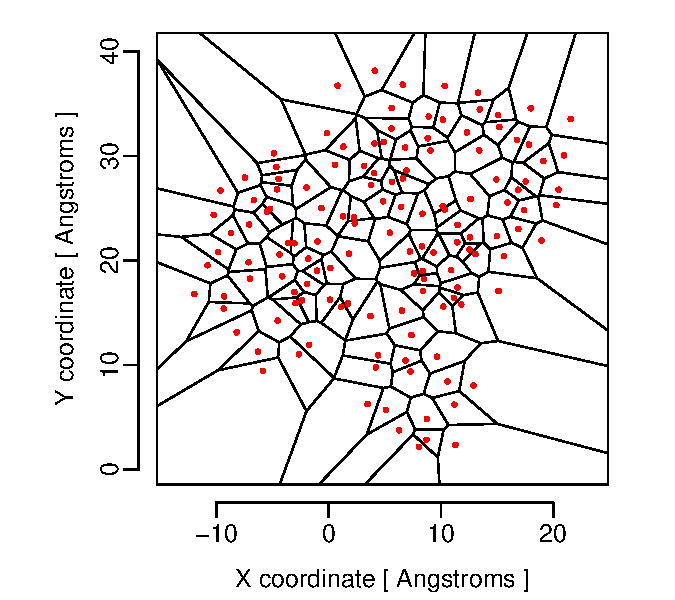
\includegraphics[width=6.9in]{voronoi_diagram.pdf}
        \end{center}
        \caption{Example 2-dimensional Voronoi diagram for bacteriophage T7 lysozyme (Protein Data Bank ID `1LBA'). The red dots represent the backbone $C_\alpha$ atoms projected on the X--Y plane, used as cell seeds in Voronoi tesellation.}
        \label{fig:voronoi}
    \end{figure}

    \begin{figure}[tbh]
        \begin{center}
        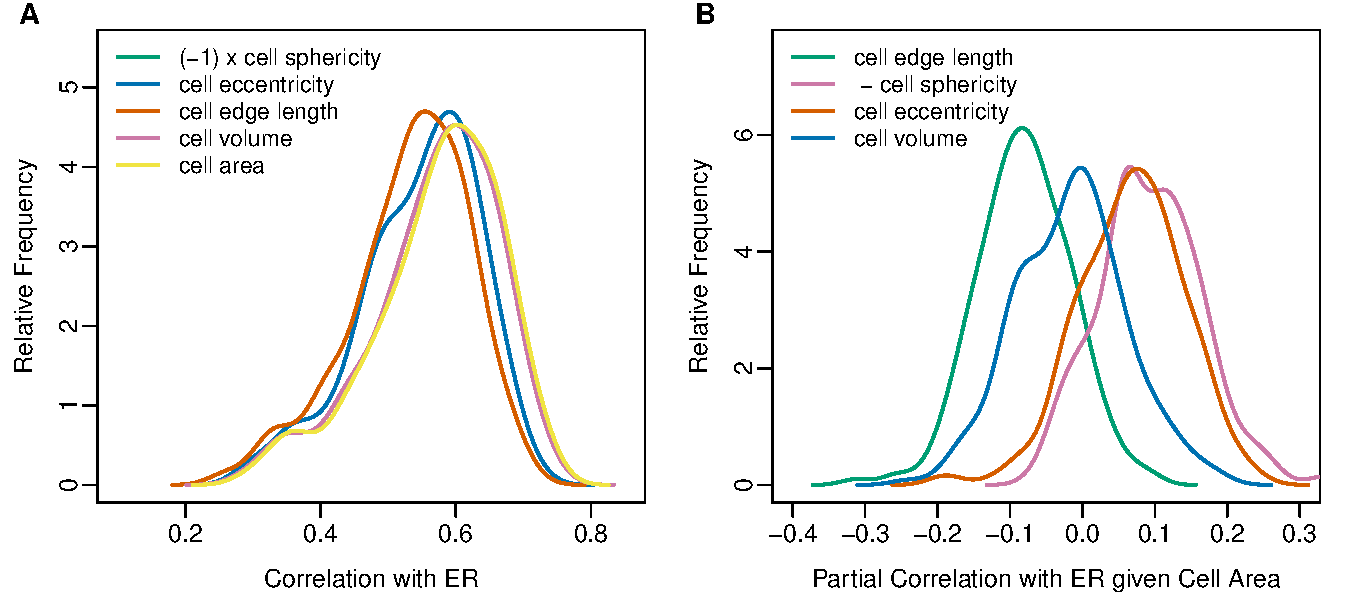
\includegraphics[width=7in]{best_voronoi_predictors_of_ER_screen.pdf}
        \end{center}
        \caption{{\bf A:} A comparison of the prediction power of different Voronoi cell characteristics about site-specific evolutionary rates (ER). Note that all cell characteristic correlate positively with ER, except sphericity which strongly negatively correlates with ER. {\bf B:} The partial correlation of the same Voronoi cell characteristics with sequence evolutionary rates while controlling for the cell area.}
        \label{fig:voronoi_ER}
    \end{figure}

    \begin{figure}[tbh]
        \begin{center}
        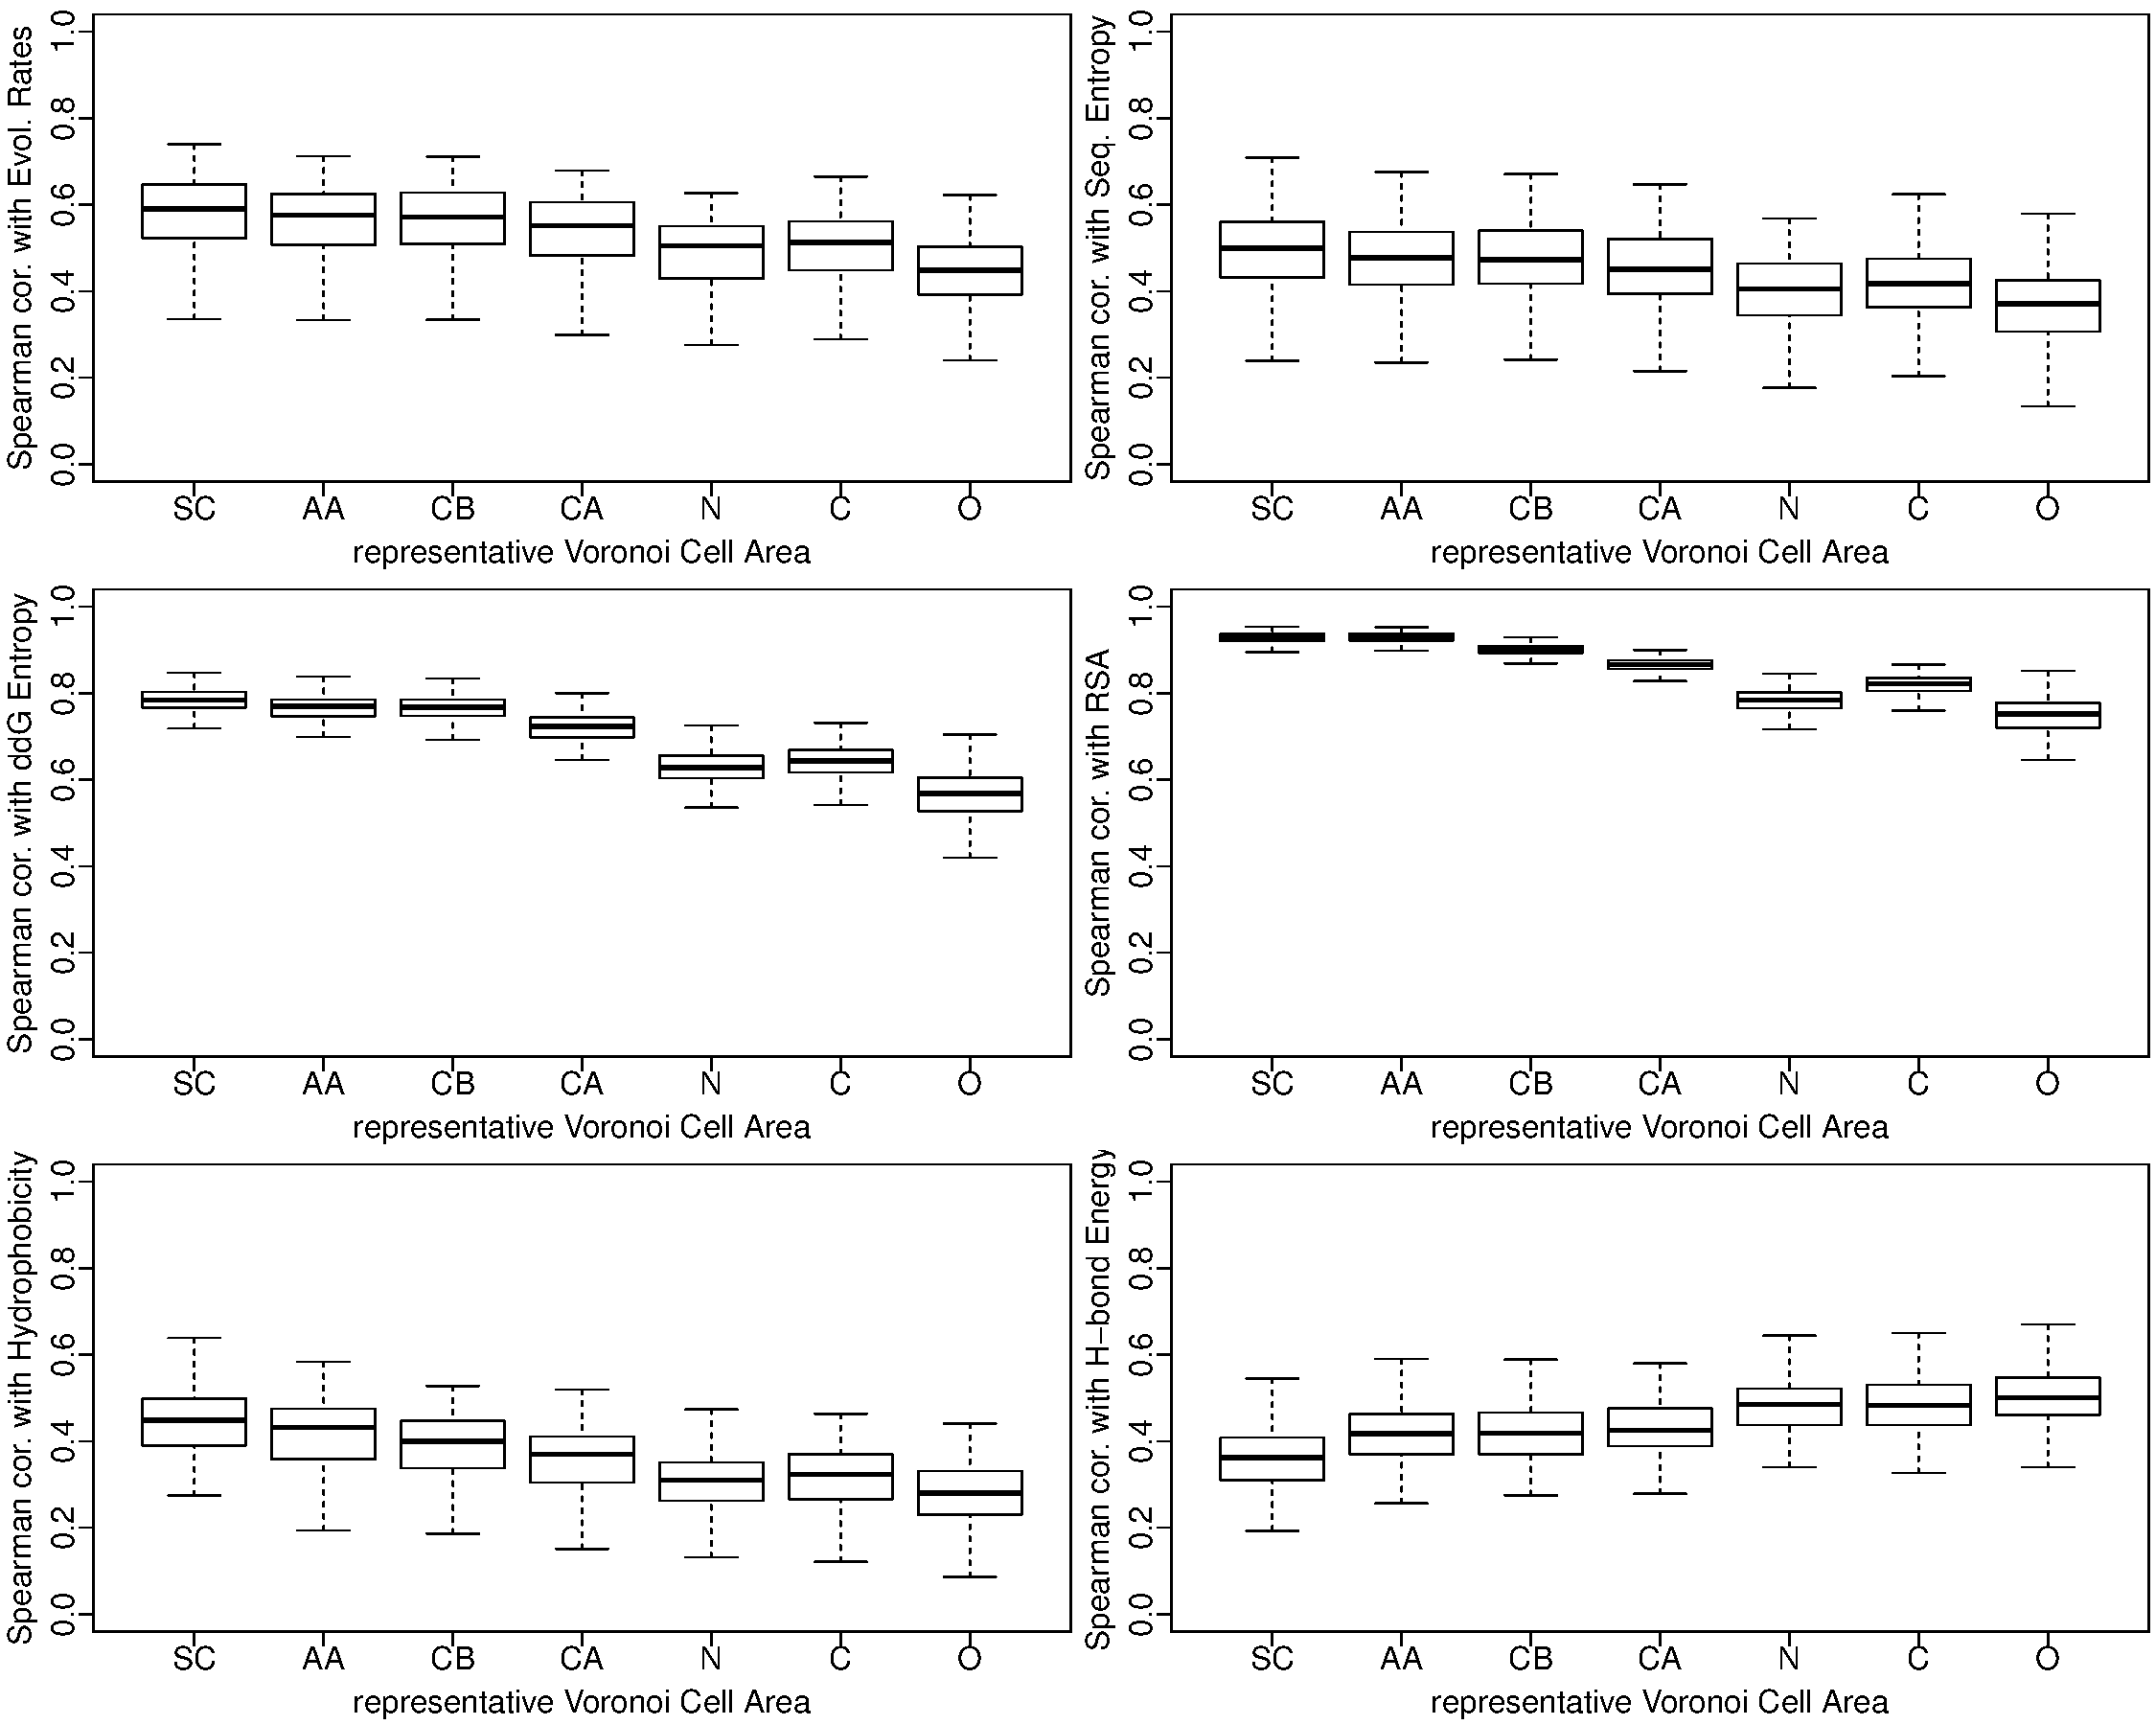
\includegraphics[width=6.9in]{best_varea/select_variables/boxplot_varea_all_in_one.pdf}
        \end{center}
        \caption{A comparison of the correlation strength of 6 different measures of Voronoi cell areas with 6 coordinate-independent structural or sequence properties for 209 proteins in dataset.  The Voronoi cells are generated using 6 sets of atomic coordinates: {\it SC, AA, CB, CA, N, C, O}, used as different representations of individual sites in proteins. The two labels {\it SC} \& {\it AA} stand respectively for the geometric average coordinates of the Side Chain (SC) atoms and the entire Amino Acid (AA) atoms, excluding hydrogens.}
        %about different structure or sequence properties for 209 proteins in dataset. In each plot, the Spearman correlation strengths of a given structure/sequence property on the vertical axis with different measures of cell areas with different atomic Voronoi seeds on the horizontal axis are compared against each other. The capital letters on the horizontal axis denote the set of atomic coordinates used in Voronoi tessellation of protein structures. }
        \label{fig:best_voronoi}
    \end{figure}


    \begin{figure}[tbh]
        \begin{center}
        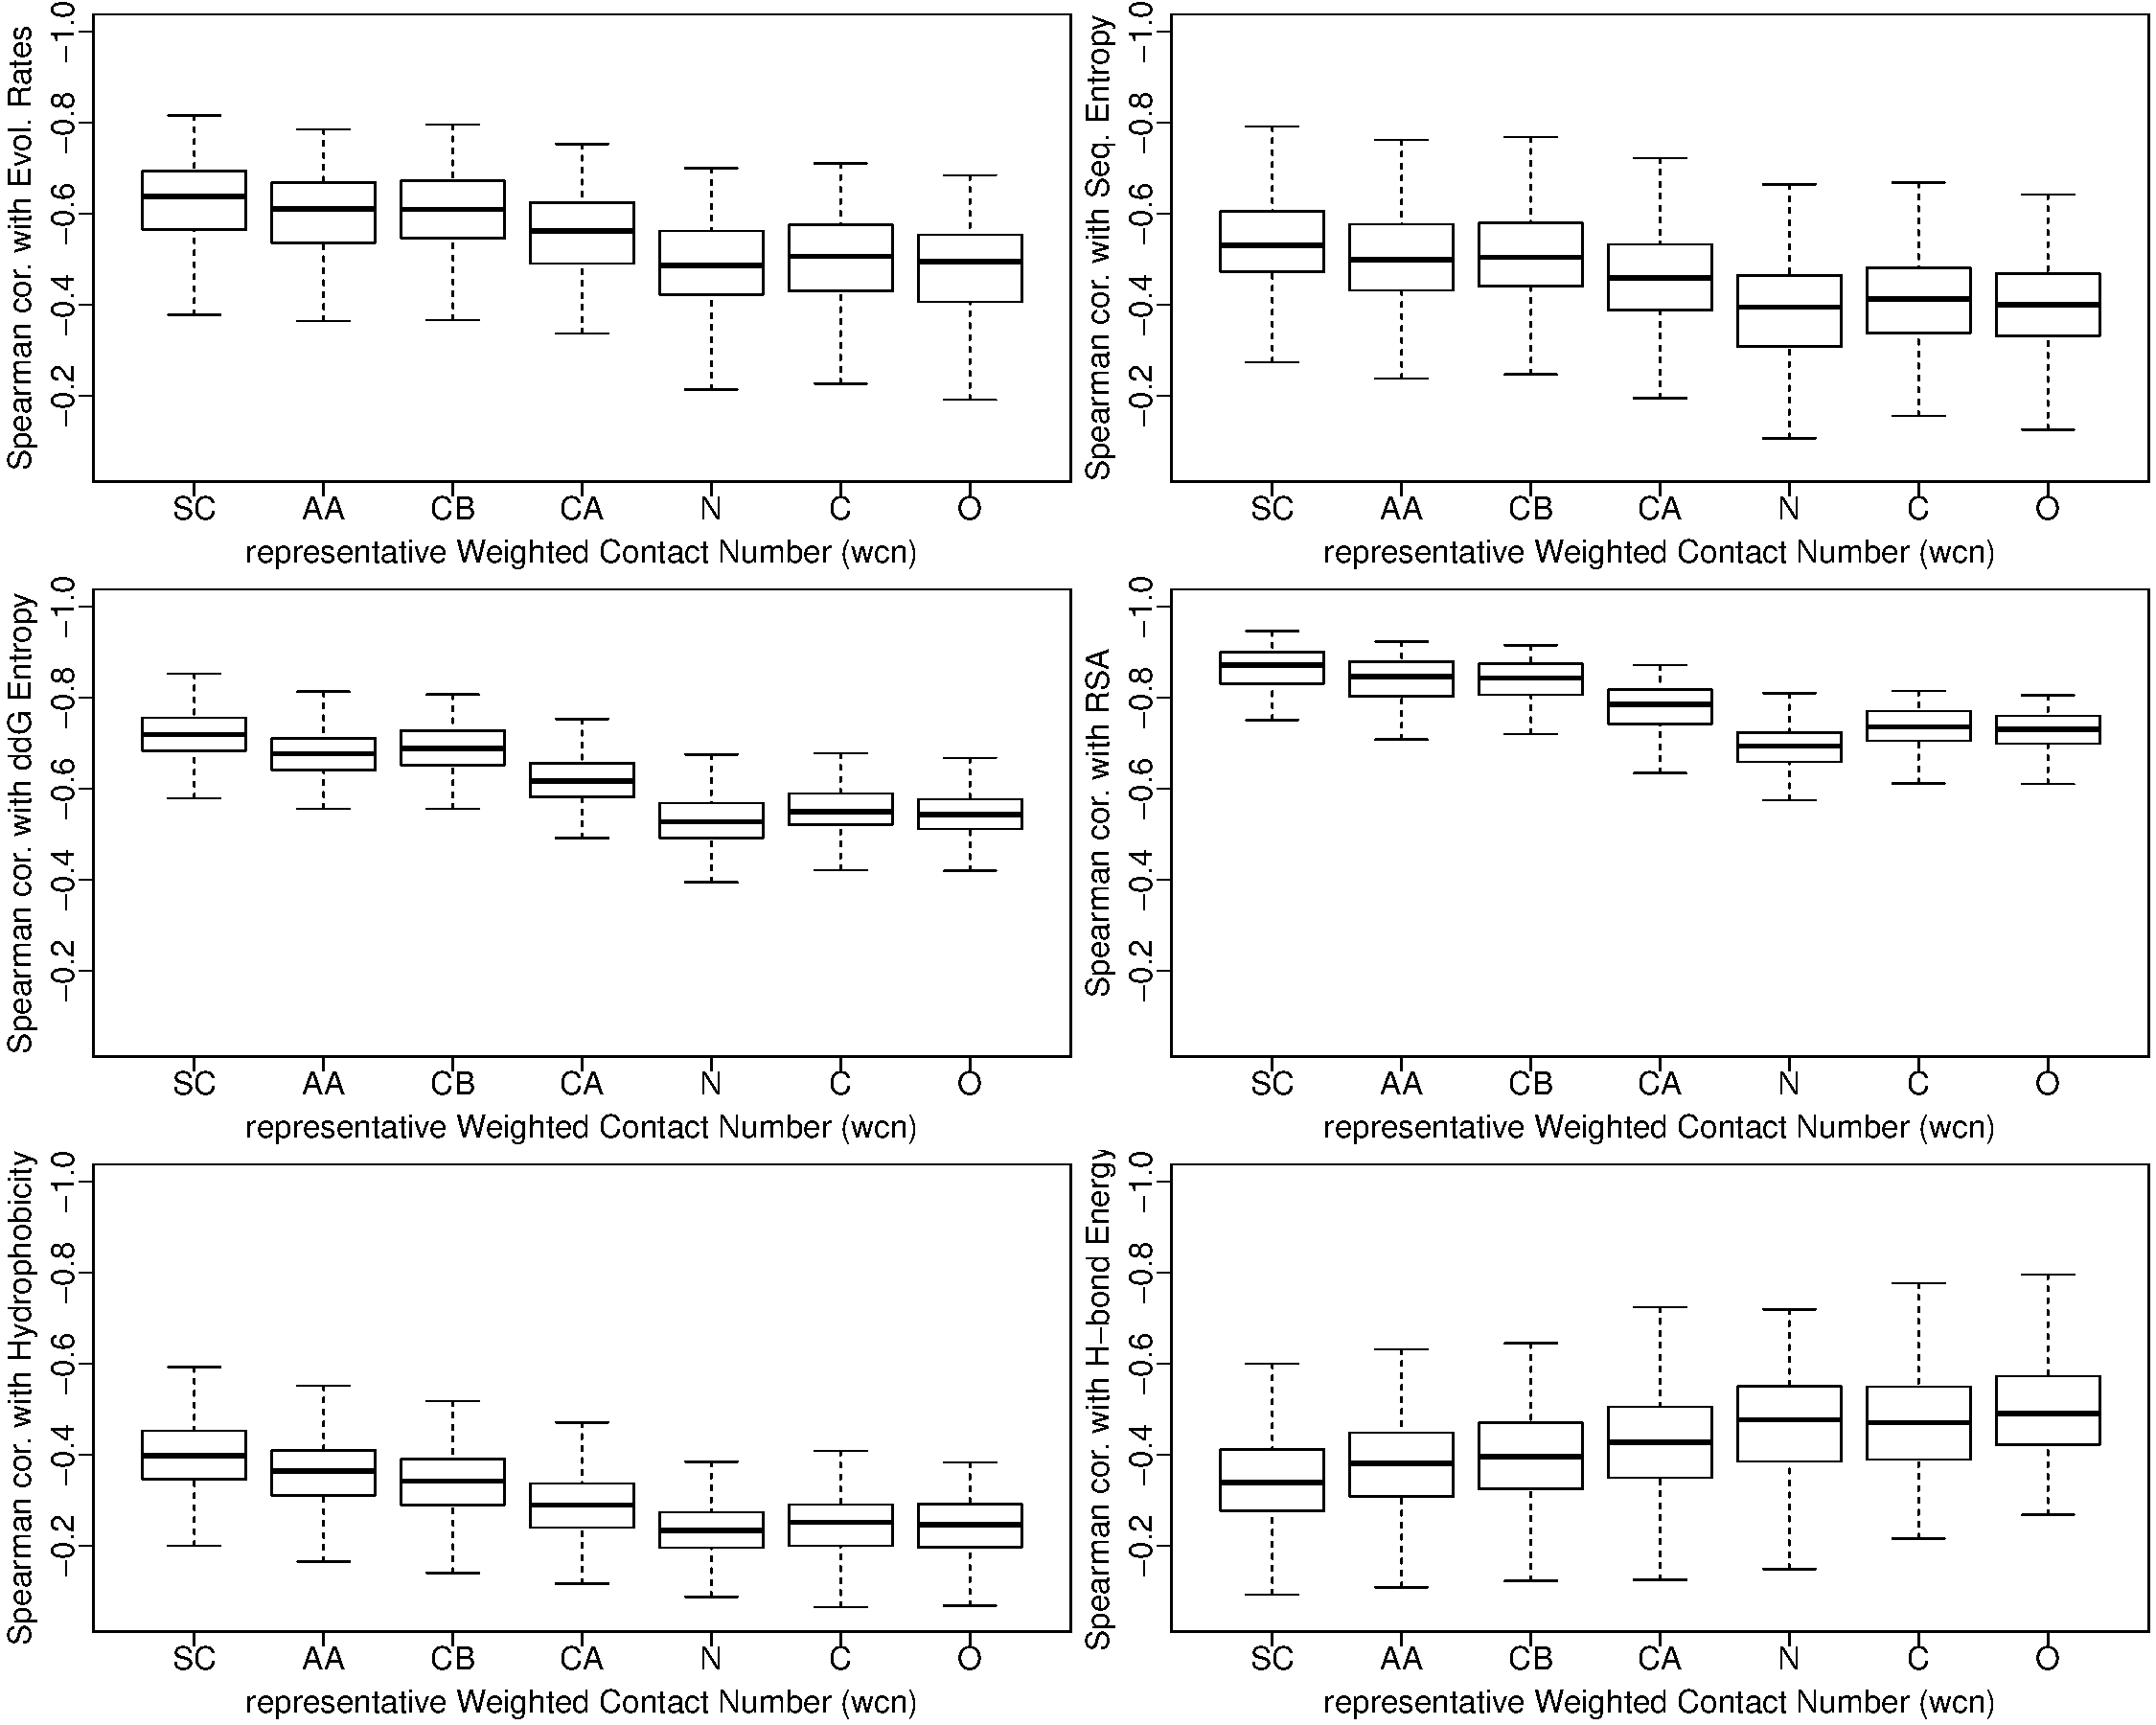
\includegraphics[width=6.9in]{best_wcn/select_variables/boxplot_wcn_all_in_one.pdf}
        \end{center}
        \caption{A comparison of the correlation strength of 6 different measures of Weighted Contact Number (WCN) with 6 coordinate-independent structural or sequence properties for 209 proteins in dataset. The contact numbers, WCN, are calculated using 6 sets of atomic coordinates: {\it SC, AA, CB, CA, N, C, O}, used as different representations of individual sites in proteins. The two labels {\it SC} \& {\it AA} stand respectively for the geometric average coordinates of the Side Chain (SC) atoms and the entire Amino Acid (AA) atoms, excluding hydrogens.}
        \label{fig:best_wcn}
    \end{figure}

    \begin{figure}[tbh]
        \begin{center}
        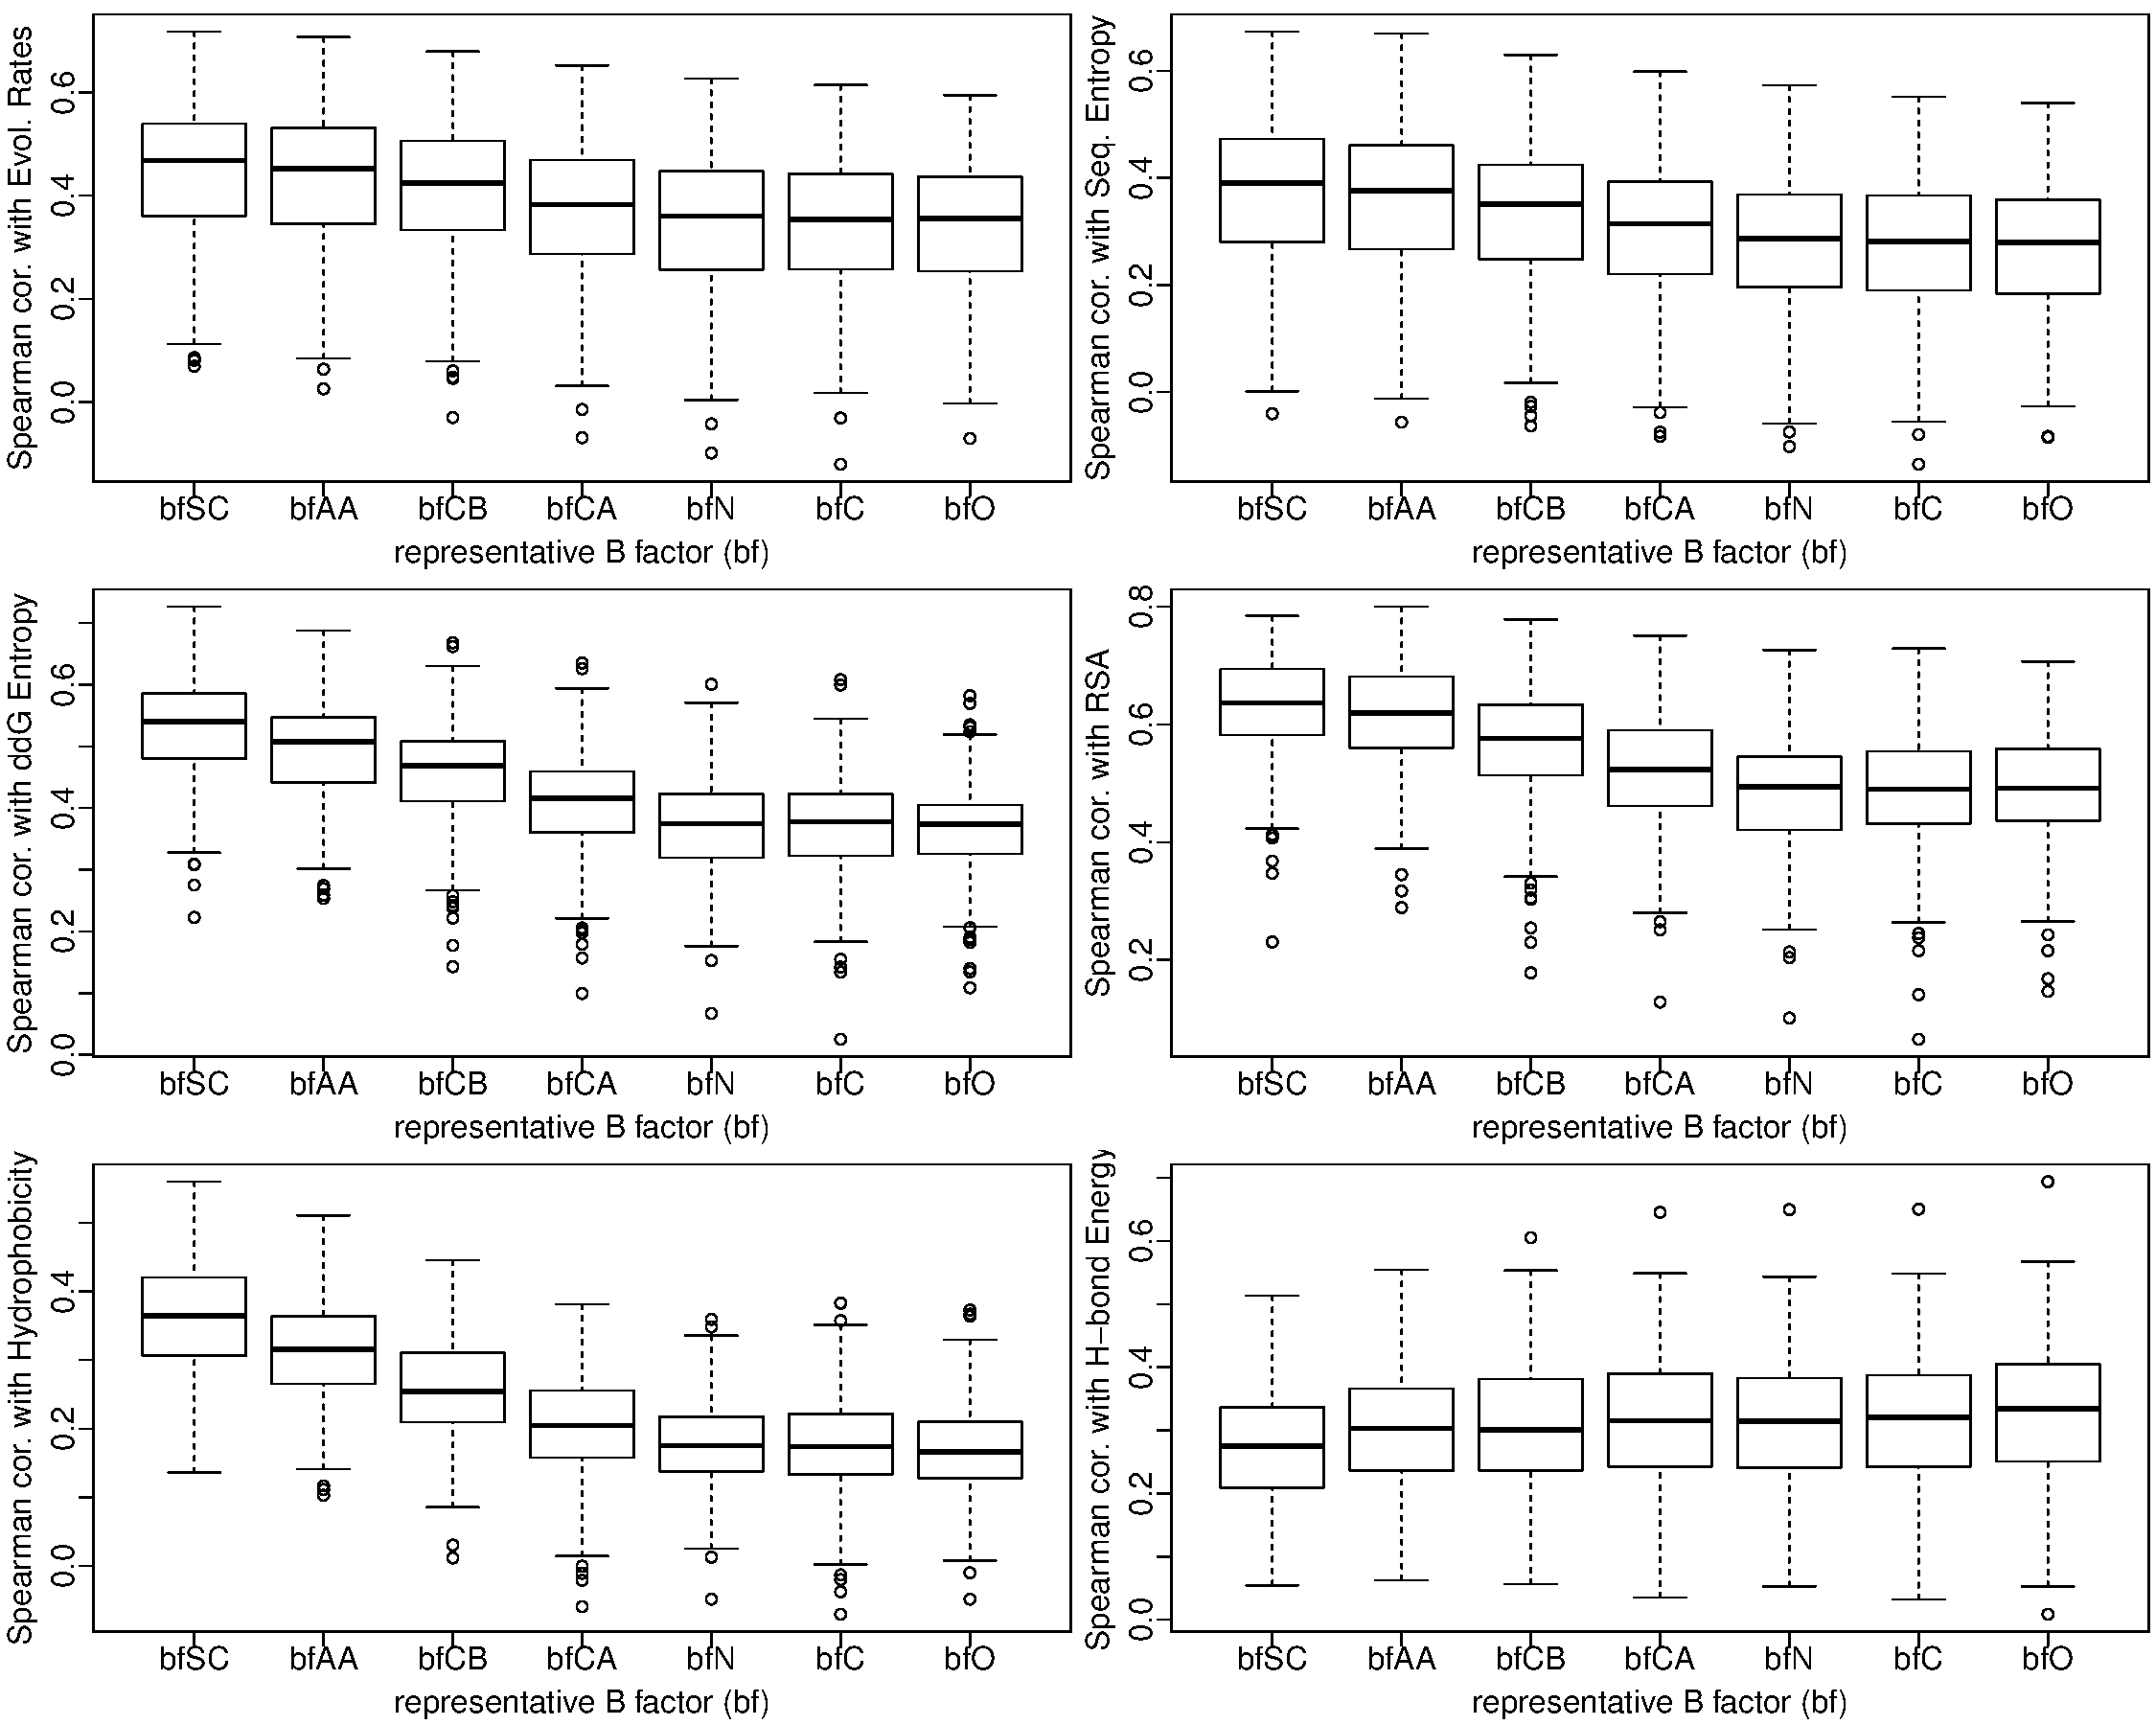
\includegraphics[width=6.9in]{best_bf/select_variables/boxplot_bf_all_in_one.pdf}
        \end{center}
        \caption{A comparison of the correlation strength of 6 different measures of B factor with 6 coordinate-independent structural or sequence properties for 209 proteins in dataset. Shown on the horizontal axes, are the 6 representative atomic B factors: {\it SC, AA, CB, CA, N, C, O} used as flexibility measures of individual sites in proteins. The two variables {\it SC} \& {\it AA} stand respectively for the average B factor of all Side Chain (SC) atoms and the entire Amino Acid (AA) atoms, excluding hydrogens.}
        \label{fig:best_bf}
    \end{figure}

    \begin{figure}[tbh]
        \begin{center}
        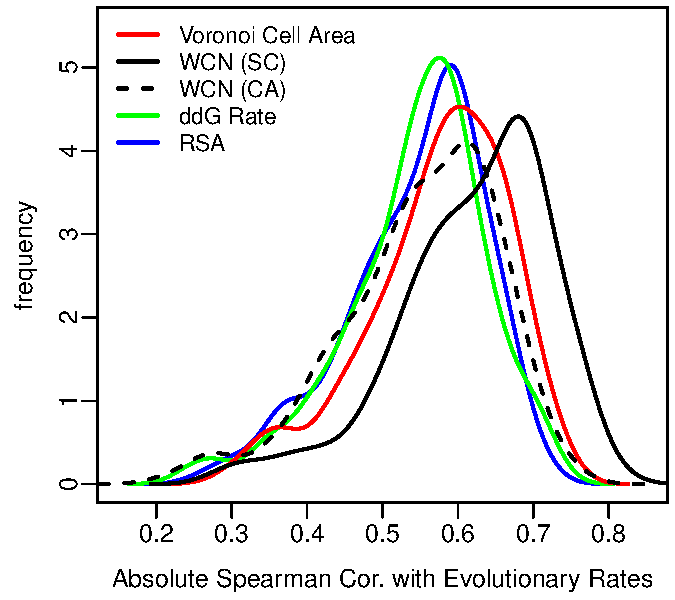
\includegraphics[width=6.9in]{best_structural_predictors_of_ER.pdf}
        \end{center}
        \caption{A comparison of the prediction power of four structural variables about site-specific evolutionary rates (ER). All structural quantities correlate positively with ER, with the exception of Weighted Contact Number (WCN) which correlates negatively. For better illustration however, the absolute Spearman's correlation of WCN with ER are shown in the Figure.}
        \label{fig:best_predictor}
    \end{figure}

%    \begin{figure}[tbh]
%        \begin{center}
%        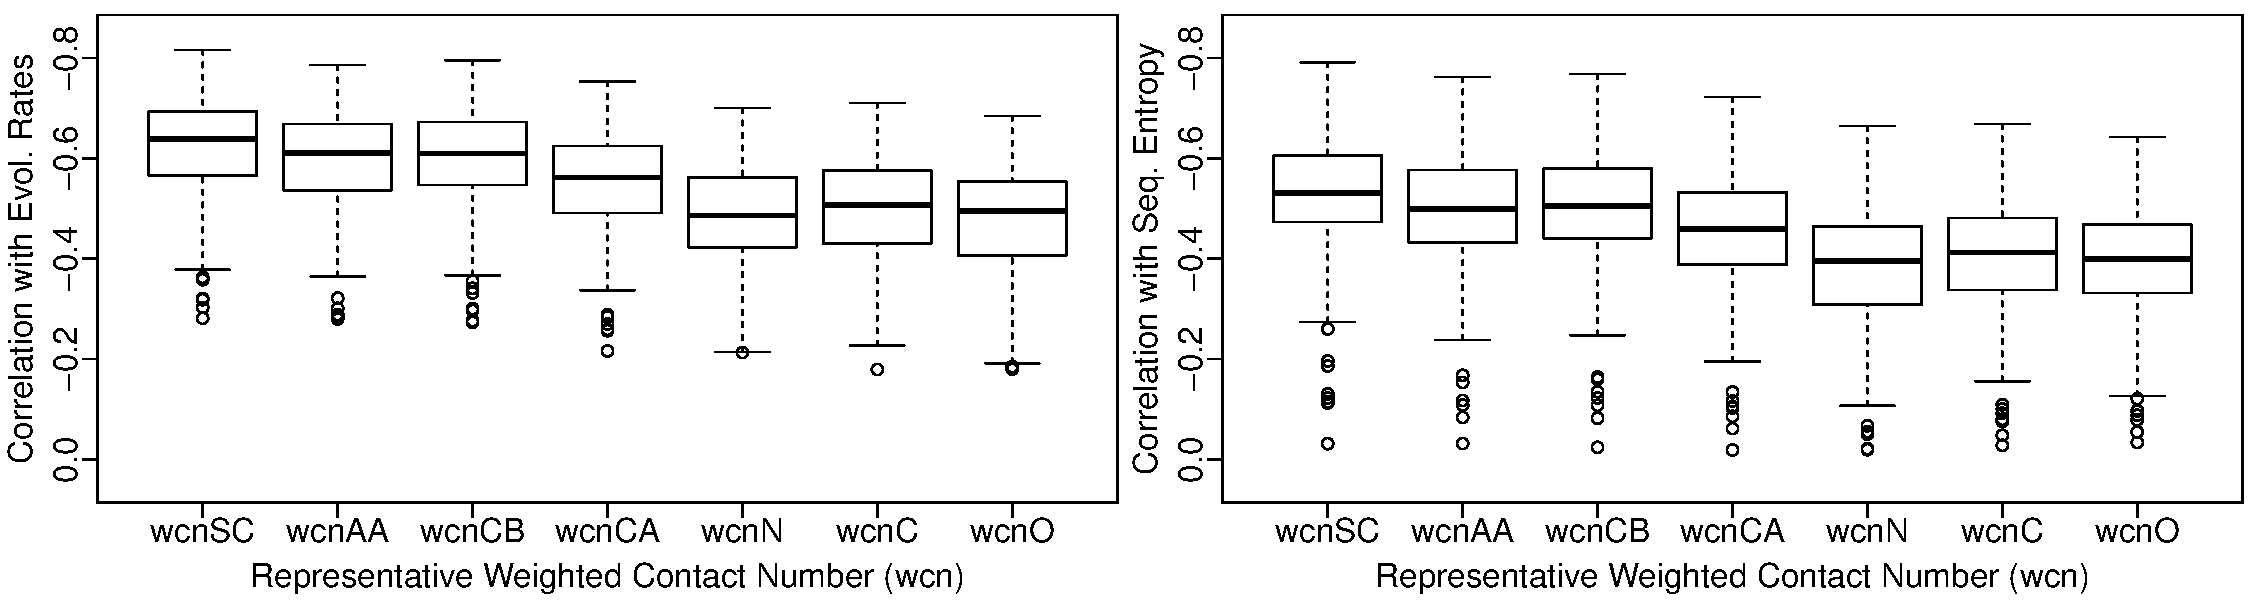
\includegraphics[width=6.9in]{best_wcn/select_variables/boxplot_wcn_two_in_one.pdf}
%        \end{center}
%        \caption{A comparison of the predictive power of different measures of Weighted Contact Number (WCN) about different structure or sequence properties for 209 proteins in dataset. In each plot, the Spearman correlation strengths of a given structure or sequence property on the vertical axis with different measures of WCN on the horizontal axis are compared against each other. The capital letters in the variable names on the horizontal axis denote the set of atomic coordinates used to calculate WCN. The variable $wcnSC$ denotes WCN measure based on the average coordinates over all heavy atoms in the side chain and the variable $wcnAA$ denotes WCN measure based on the average coordinate over all heavy atoms in the side chain and backbone of the amino acid.}
%        \label{fig:best_wcn}
%    \end{figure}

\bibliographystyle{mbe}
\bibliography{mnv}

\end{document}

